\documentclass[conference]{IEEEtran}
\IEEEoverridecommandlockouts
% The preceding line is only needed to identify funding in the first footnote. If that is unneeded, please comment it out.
\usepackage{cite}
\usepackage[utf8]{inputenc}
\usepackage{amsmath,amssymb,amsfonts}
\usepackage{algorithmic}
\usepackage{graphicx}
\usepackage{textcomp}
\usepackage[portuguese]{babel}
\usepackage{xcolor}
\def\BibTeX{{\rm B\kern-.05em{\sc i\kern-.025em b}\kern-.08em
    T\kern-.1667em\lower.7ex\hbox{E}\kern-.125emX}}
\begin{document}


\title{Aplicação de uma Rede Neural MLP de Classificação para Identificação de Subtipos de Doenças Eritematoescamosas em Dermatologia\\
}

\author{\IEEEauthorblockN{André Dias Neto}
\IEEEauthorblockA{\textit{Engenharia de Computação} \\
\textit{Instituto Federal de Minas Gerais}\\
Bambuí, Brasil \\
andre1parallel@gmail.com}
\and
\IEEEauthorblockN{Letícia Moreira Leonel}
\IEEEauthorblockA{\textit{Engenharia de Computação} \\
\textit{Instituto Federal de Minas Gerais}\\
Bambuí, Brasil \\
leticiamoreiraleonel0318@gmail.com}
}

\maketitle

\begin{abstract}
Neste trabalho, apresentamos os resultados da implementação de uma rede neural MLP (Multi-Layer Perceptron) para classificação de subtipos de Doença Eritematoescamosa em um banco de dados dermatológico. A Doença Eritematoescamosa é uma condição dermatológica comum, caracterizada por eritema e descamação da pele. O diagnóstico preciso dessa doença é crucial para o tratamento adequado dos pacientes. Utilizamos uma abordagem baseada em aprendizado de máquina, aproveitando os benefícios das redes neurais artificiais para melhorar a precisão e a automatização do diagnóstico.
\end{abstract}

\begin{IEEEkeywords}
Doença Eritematoescamosa, classificação, redes neurais artificiais, MLP, aprendizado de máquina, dermatologia.
\end{IEEEkeywords}

\section{Introdução}
A classificação precisa e rápida de doenças dermatológicas é essencial para o diagnóstico e tratamento eficazes. A Doença Eritematoescamosa, Figura \ref{fig:doenca}, é uma condição comum que se caracteriza por eritema e descamação da pele. Neste trabalho, propomos a implementação de uma rede neural MLP (Multi-Layer Perceptron) para classificar o tipo de Doença Eritematoescamosa com base em um banco de dados dermatológico.

\begin{figure}[htbp]
    \centerline{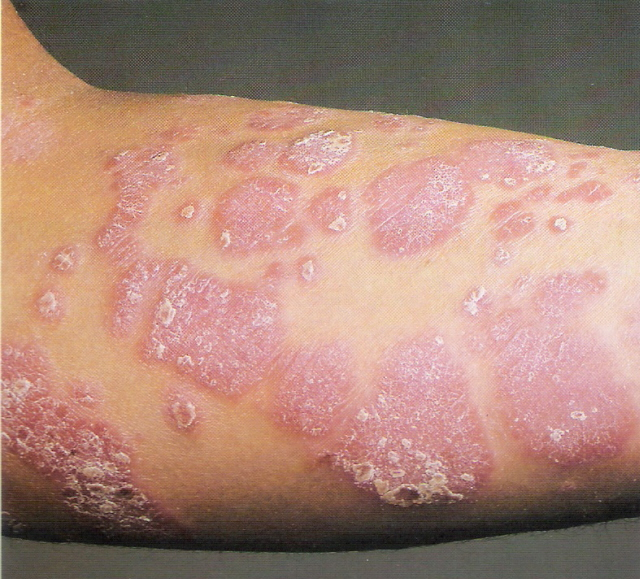
\includegraphics{./figuras/figura1.jpg}}
    \caption{Exemplo de doença eitematoescamosa}
    \label{fig:doenca}
\end{figure}

O conjunto de dados construído para este domínio contém informações relevantes, como o atributo de histórico familiar, que indica se alguma dessas doenças foi observada na família, e o recurso de idade, que representa a idade do paciente. Além disso, todas as outras características clínicas e histopatológicas foram avaliadas em uma escala de 0 a 3, onde 0 indica a ausência da característica, 3 indica a maior quantidade possível e 1 e 2 representam valores intermediários relativos. Este banco de dados pronto foi forncecido pelo site Kaggle, e através do link (https://www.kaggle.com/datasets/olcaybolat1/dermatology-dataset-classification) pode-se ter acesso a ele.

A rede neural MLP é uma escolha adequada para a tarefa de classificação, pois é capaz de aprender relações complexas entre as características dos pacientes e suas respectivas classes. Através do treinamento da rede utilizando dados rotulados, buscamos criar um modelo capaz de reconhecer padrões discriminatórios e realizar a classificação automatizada dos diferentes tipos de Doença Eritematoescamosa.

Com isso, em busca de trabalhos que utilizassem este banco de dados específico, encontramos um que faz a comparação de vários classificadores [1], dentre eles a MLP. Com isso, decidimos fazer uma implementação específica da MLP para comparar os resultados de acurácia com o trabalho que encontramos. 

Esperamos que a implementação da rede neural MLP neste contexto dermatológico traga benefícios significativos, fornecendo uma ferramenta confiável para auxiliar médicos e dermatologistas no diagnóstico precoce e no tratamento personalizado da Doença Eritematoescamosa. Além disso, a análise de características clínicas, histopatológicas e informações de histórico familiar permitirá uma abordagem abrangente e aprimorada no entendimento dessa condição dermatológica comum.

\section{Caracterização do Problema e trabalhos relacionados}
A classificação precisa e automatizada do tipo de Doença Eritematoescamosa com base em características clínicas e histopatológicas é um desafio importante na área dermatológica. Identificar corretamente o tipo de doença é fundamental para orientar o tratamento adequado e melhorar a qualidade de vida dos pacientes. 

Vários trabalhos têm se dedicado ao desenvolvimento de abordagens para a classificação de doenças dermatológicas, incluindo a Doença Eritematoescamosa. Alguns estudos têm explorado métodos tradicionais de aprendizado de máquina, como árvores de decisão, redes Bayesianas e SVM (Support Vector Machines), utilizando características clínicas e histopatológicas para realizar a classificação. Essas abordagens têm obtido resultados promissores, mas ainda enfrentam desafios relacionados à precisão e eficiência.

A. Boçois \textit{et al.} (2012) fizeram um estudo que teve como objetivo demonstrar a possibilidade de desenvolver um software de diagnóstico utilizando redes neurais artificiais para auxiliar na detecção e diagnóstico de doenças dermatológicas, sendo o diagnóstico final do médico responsável. Os autores concluíram que o modelo proposto obteve uma aproximação satisfatória entre os resultados da rede neural e os resultados esperados, e que com aperfeiçoamento e utilização de outras técnicas é viável a utilização da ferramenta como auxílio à tomada de decisão médica de forma eficiente.

O autor P. Gamarra Lessa Pinto (2019) apresentou um método baseado em redes neurais convolucionais para classificação de imagens dermatológicas de lesões de pele, com o objetivo de desenvolver um sistema para auxiliar profissionais da saúde na detecção de doenças dermatológicas. O método utilizado foi treinado utilizando uma base de dados rotulada por profissionais da área, e os dados foram divididos em 75\% para treino e 25\% para teste. O autor concluiu que o modelo apresentou resultados satisfatórios, superando em alguns aspectos outros trabalhos utilizados como estado da arte.

V. A. Gulartt e R. Luiz Antoniazzi (2021) fizeram a utilização das bibliotecas OpenCV, Keras e Tensorflow, e implementaram uma rede neural convolunional que foi treinada utilizando imagens de melanoma cutâneo e nevos comuns (pequenas lesões cutâneas) para identificação de padrões existentes nas imagens. Foram utilizadas 130 imagens para o treinamento, divididas em três grupos, o primeiro com imagens de nevos melanócitos (popularmente conhecido como pintas), o segundo com imagens de tumores do tipo carcinoma basocelular e o terceiro por imagens de melanoma cutâneo. Os conjuntos foram divididos em 60\% para o treino, 20\% para o conjunto validação e 20\% para o conjunto de teste. Os autores concluíram que a utilização de uma rede neural convolucional para detecção de padrões em imagens se prova útil quando o treinamento da rede é realziado a partir de parâmetros corretos e com uma base de dados de entrada suficientemente grande para satisfazer os requisitos de treinamento da rede.

Além disso, recentemente, houve um interesse crescente na aplicação de técnicas de aprendizado profundo, especialmente redes neurais convolucionais (CNNs), para a classificação de doenças dermatológicas. Em comparação com outros algoritmos de classificação, uma CNN exige muito menos pré-processamento, e com treinamento suficiente as CNNs tem capacidade de aprender filtros e características, não sendo necessária a criação manual como em métodos primitivos (OLIVEIRA, 2019). No entanto, a aplicação direta de CNNs para a classificação da Doença Eritematoescamosa ainda é um campo em desenvolvimento, e é importante explorar outras arquiteturas de redes neurais, como a MLP, que podem ter vantagens específicas para esse problema.

Embora haja trabalhos relevantes sobre a classificação de doenças dermatológicas, poucos se concentraram especificamente na Doença Eritematoescamosa e no uso da rede neural MLP para essa tarefa. Portanto, este estudo visa preencher essa lacuna ao implementar e avaliar uma rede neural MLP para a classificação precisa e automatizada dos subtipos dessa doença.

Ao explorar os trabalhos relacionados, buscamos identificar as abordagens existentes, suas limitações e os avanços alcançados até o momento. Isso nos permite compreender o estado da arte, identificar oportunidades de melhoria e posicionar nosso trabalho em relação aos estudos anteriores, contribuindo para o avanço do campo de diagnóstico de doenças dermatológicas, em particular, a Doença Eritematoescamosa.

\section{Fundamentação Teórica}
As redes neurais artificiais (RNAs) têm suas origens em pesquisas realizadas desde a década de 1940, quando McCulloch e Pitts propuseram o primeiro modelo de neurônio artificial, inspirado nos neurônios biológicos e no sistema nervoso. No entanto, atualmente, esses dois sistemas não possuem grandes semelhanças (BARRETO, 2002).

De acordo com Barreto (2002), uma rede neural artificial pode ser entendida como uma abordagem para resolver problemas de inteligência artificial (IA).

Barreto (2002) enfatiza que o objetivo de uma RNA é construir circuitos neurais artificiais que possam se auto-organizar e, diante de ambientes diversos, serem capazes de aprender novas tarefas, cometer erros, fazer generalizações e descobertas, tornando-se um sistema com comportamento inteligente.

Esses sistemas de RNA são considerados como sistemas paralelos e distribuídos, uma vez que a estrutura das RNAs é constituída por um conjunto de neurônios interconectados trabalhando simultaneamente para processar dados (ROSSINI; CAMOLESI, 2018).

Uma rede neural convolucional (CNN) é um algoritmo de deep learning (aprendizado
profundo) que pode captar uma imagem, atribuir importância a vários objetos e aspectos da
imagem sendo capaz de diferenciá-los. Em comparação com outros algoritmos de
classificação, uma CNN exige muito menos pré-processamento, com treinamento suficiente
as CNNs tem capacidade de aprender filtros e características, não sendo necessária a criação
manual como em métodos primitivos. Sua arquitetura é similar à do padrão de conectividade
de neurônios no cérebro humano, e inspirada na organização visual do córtex cerebral (DEEP LEARNING BOOK, 2022).

A implementação proposta por este trabalho utiliza uma Rede Neural Artificial (RNA) do tipo Multi-Layer Perceptron (MLP) para realizar a classificação de doenças eritematoescamosas em um banco de dados dermatológico.

Uma rede MLP Figura \ref{fig:mlp} é uma das arquiteturas mais comumente utilizadas em RNAs. Consiste em uma rede formada por múltiplas camadas de neurônios, com pelo menos uma camada intermediária. O MLP é composto por uma camada de entrada, uma ou mais camadas ocultas e uma camada de saída. Cada neurônio em uma camada está conectado a todos os neurônios da camada seguinte por meio de conexões sinápticas ponderadas. As redes MLP possuem diversas possibilidades de aplicações nos mais variados problemas relacionados com as mais diferentes áreas de conhecimento, sendo considerada uma das arquiteturas mais versáteis quanto a sua aplicabilidade  (DA SILVA; SPATTI; FLAUZINO, 2010).

\begin{figure}[htbp]
    \centerline{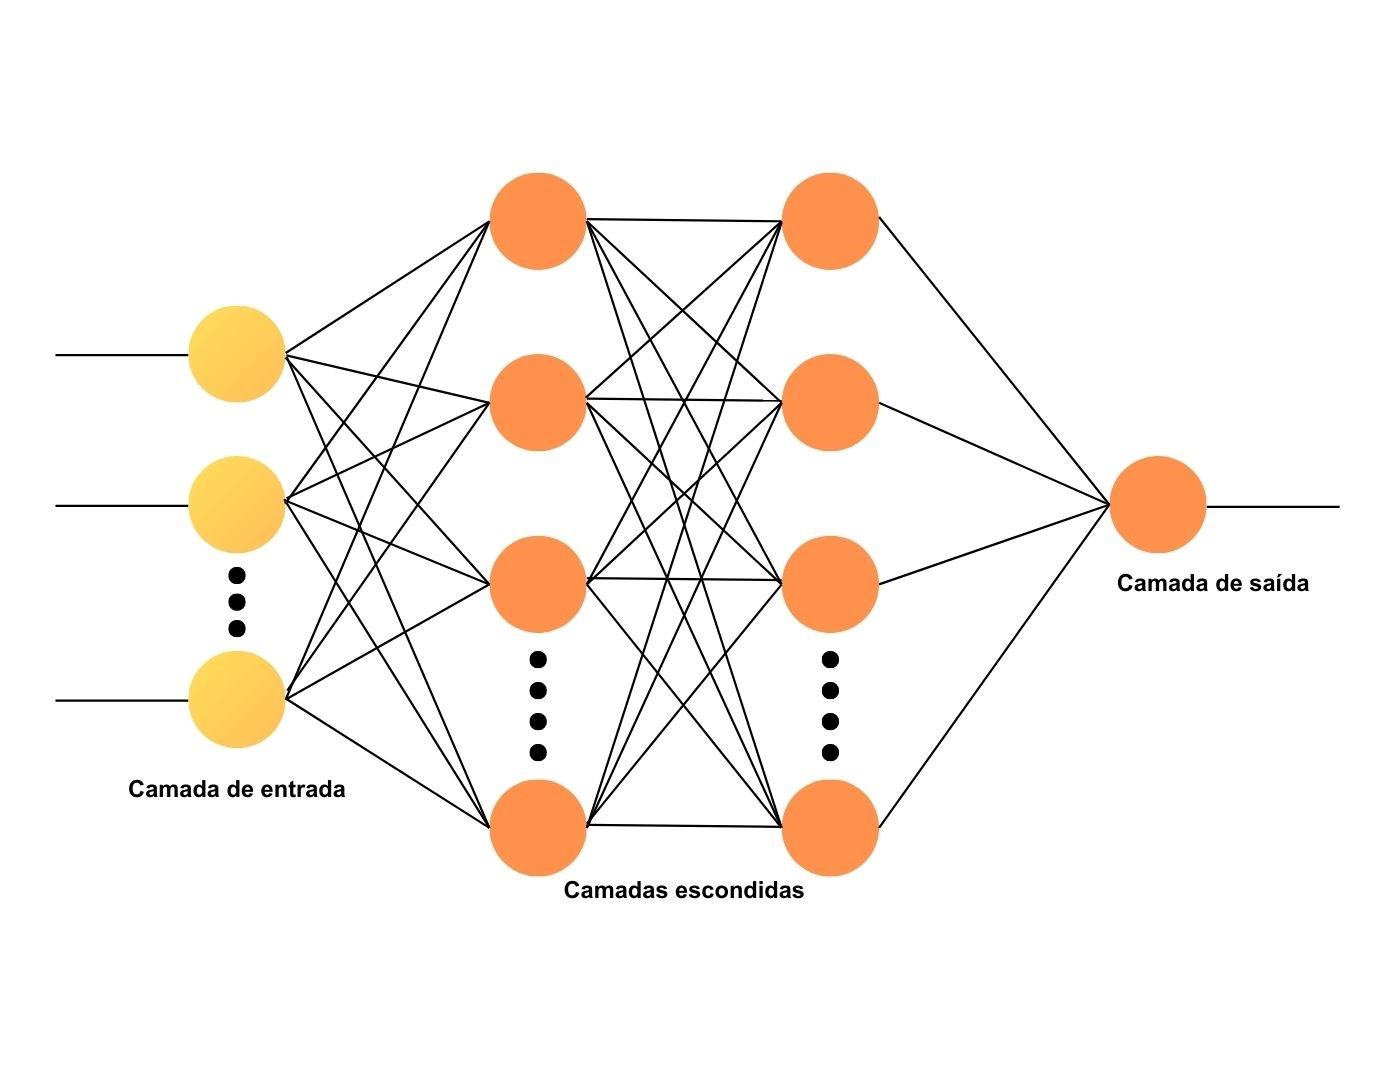
\includegraphics[width = 1.0\linewidth]{./figuras/figura2.jpg}}
    \caption{Arquitetura MLP}
    \label{fig:mlp}
\end{figure}

No problema de classificação em questão, o MLP utiliza as características dermatológicas como entrada (como dados de sintomas, medidas etc.) e realiza o aprendizado supervisionado para determinar o tipo de doença eritematoescamosa correspondente. Durante o treinamento, os pesos sinápticos são ajustados iterativamente para minimizar uma função de perda, usando o algoritmo de retropropagação do erro.

Diferentemente de outros algoritmos clássicos de aprendizado de máquina, como árvores de decisão ou regressão logística, o MLP possui capacidade de aprendizado em problemas complexos, não lineares e com múltiplas classes. Ele é capaz de aprender representações não lineares dos dados por meio das camadas ocultas, que introduzem não linearidades através de funções de ativação (GOODFELLOW; BENGIO; COURVILLE, 2016).

Algumas diferenças notáveis entre o MLP e outros algoritmos incluem:

1. Flexibilidade: O MLP pode aprender funções não lineares complexas, permitindo a modelagem de problemas mais complexos e com maior poder de representação (DA SILVA, 2017).

2. Treinamento iterativo: O MLP utiliza o algoritmo de retropropagação do erro para ajustar os pesos sinápticos durante o treinamento. Isso permite que ele aprenda a partir dos erros cometidos na classificação e refine seus parâmetros ao longo do tempo (GOODFELLOW; BENGIO; COURVILLE, 2016).

3. Camadas ocultas: O MLP pode ter uma ou mais camadas ocultas, o que lhe confere a capacidade de aprender representações intermediárias dos dados. Essas camadas ocultas permitem que a rede capture relações complexas e abstrações de alto nível dos recursos de entrada (CHOLLET, 2018).

4. Generalização: O MLP tem a capacidade de generalizar a partir dos exemplos de treinamento para classificar corretamente novos exemplos que não foram vistos durante o treinamento. Isso é possível devido ao processo de ajuste dos pesos sinápticos e ao uso de funções de ativação não lineares (HAYKIN, 2009).

É importante ressaltar que o desempenho do MLP depende da adequada seleção dos hiperparâmetros, como o número de neurônios em cada camada oculta, a taxa de aprendizado, a função de ativação e o número de épocas de treinamento. Esses hiperparâmetros podem ser ajustados empiricamente ou por meio de técnicas de otimização, como busca em grade ou busca aleatória.

No contexto deste trabalho, realizamos o pré-processamento dos dados, normalizando-os e tratando valores ausentes. Em seguida, dividimos os dados em conjuntos de treinamento e teste. Utilizamos a biblioteca scikit-learn para criar uma instância de MLPClassifier, configurando seus parâmetros. Em seguida, treinamos a rede neural usando o conjunto de treinamento e avaliamos sua acurácia usando o conjunto de teste.

Além disso, também realizamos a predição de novos dados utilizando o modelo treinado e plotamos gráficos para visualizar as previsões em comparação com as classes reais. Também calculamos e exibimos a matriz de confusão e as métricas de avaliação, como acurácia, precisão, recall e F1-score para cada classe.

Essa é uma abordagem poderosa para a classificação de doenças eritematoescamosas e permite automatizar a tarefa de diagnóstico com base em características dermatológicas. O MLP tem a capacidade de aprender padrões complexos nos dados e realizar classificações precisas, desde que seja adequadamente treinado e configurado.

\section{Metodologia}
A metodologia envolveu o processamento dos dados, configuração e treinamento do modelo MLP, avaliação do modelo e análise dos resultados obtidos. O algoritmo MLPClassifier foi adaptado ao problema específico de classificação de doenças eritematoescamosas, e o conjunto de dados foi modelado para se adequar às exigências do algoritmo, permitindo o treinamento e a avaliação do modelo. Abaixo temos a explicação de cada passo:

1. Preparação dos dados:
   - Carregamento do conjunto de dados: Os dados dermatológicos foram carregados a partir de um arquivo CSV.
   - Tratamento de dados ausentes: Foram identificados valores ausentes representados por "?", que foram substituídos por "Not a Number".
   - Conversão dos dados para numéricos: Os dados foram convertidos para o tipo float.
   - Preenchimento dos valores ausentes: Os valores ausentes foram preenchidos com a média dos respectivos atributos.
   - Separação dos recursos e variável alvo: Os recursos de entrada foram separados em uma variável, enquanto a variável alvo (classe) foi atribuída a outra variável.

2. Pré-processamento dos dados:
   - Normalização dos dados: Os dados de entrada foram normalizados para evitar que atributos com diferentes escalas afetem o desempenho do modelo.

3. Divisão dos dados:
   - Divisão em conjunto de treinamento e teste: Os dados foram divididos em um conjunto de treinamento e um conjunto de teste. O conjunto de teste foi utilizado para avaliar o desempenho do modelo após o treinamento da RNA.

4. Criação e treinamento da Rede Neural MLP:
   - Configuração do MLPClassifier: Foi criada uma instância do MLPClassifier com parâmetros definidos, como o número de camadas ocultas, o número de neurônios em cada camada, o número máximo de iterações (épocas) e a taxa de aprendizado.
   - Treinamento do MLP: A rede neural foi treinada utilizando os dados de treinamento, ajustando os pesos e o bias para encontrar os melhores parâmetros para a classificação.

5. Avaliação do modelo:
   - Previsão e acurácia: A partir dos dados de teste, foram feitas previsões utilizando o modelo treinado. A acurácia foi calculada comparando as previsões com as classes reais, fornecendo uma medida de quão bem o modelo é capaz de classificar corretamente os dados de teste.
   - Curva de Acurácia: Foi plotada uma curva de acurácia para visualizar como a acurácia do modelo evoluiu durante o treinamento.

6. Análise e visualização dos resultados:
   - Gráfico de comparação de classes previstas vs. classes reais: Foi plotado um gráfico de dispersão para comparar as classes previstas pelo modelo com as classes reais. Isso permite visualizar como as previsões se aproximam dos valores reais.
   - Gráfico de comparação de dados reais e previstos: Foi plotado um gráfico de dispersão para comparar os dados reais e previstos em relação a um dos atributos. Isso ajuda a verificar se o modelo está capturando corretamente as relações entre os atributos e as classes.
   - Matriz de confusão: Foi calculada e plotada uma matriz de confusão para avaliar o desempenho do modelo em termos de verdadeiros positivos, verdadeiros negativos, falsos positivos e falsos negativos.
   - Tabela de Métricas de Avaliação: Foi gerada uma tabela contendo métricas de avaliação, como precisão, recall e F1-score, para cada classe. Isso fornece uma análise mais detalhada do desempenho do modelo em cada classe.

\section{Resultados}
Os resultados forneceram informações importantes sobre o desempenho e a qualidade do modelo de classificação MLP para o problema de determinação do tipo de doença eritematoescamosa no banco de dados dermatológico. Eles foram utilizados para avaliar a eficácia do modelo e identificar possíveis melhorias.

Os seguintes resultados foram obtidos:

1. Acurácia do modelo:
   - A acurácia do modelo MLP foi calculada utilizando a função 'accuracy-score da biblioteca scikit-learn. A acurácia mede a conformidade de exemplos classificados corretamente em relação ao total de exemplos. No caso desse modelo, a acurácia representa a taxa de classificação correta das doenças eritematoescamosas no conjunto de teste. Com isso, obtivemos a taxa de 0.96 de acurácia em nosso modelo implementado.

2. Curva de Acurácia:
   - A curva de acurácia Figura \ref{fig:acuracia} foi plotada utilizando a lista de acurácias obtidas em cada época durante o treinamento do modelo. Esse gráfico mostra como a acurácia do modelo evoluiu ao longo das épocas de treinamento.

\begin{figure}[htbp]
    \centerline{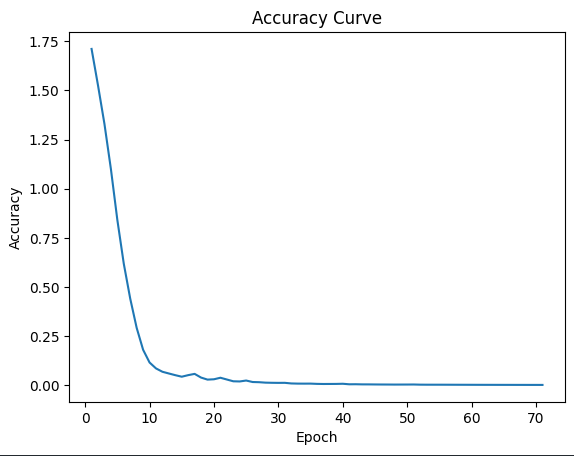
\includegraphics[width = 1.0\linewidth]{./figuras/figura3.png}}
    \caption{Gráfico que representa a curva da acurácia}
    \label{fig:acuracia}
\end{figure}

3. Gráfico de comparação de classes previstas vs. classes reais:
   - Foi plotado um gráfico de dispersão para comparar as classes previstas pelo modelo com as classes reais Figura \ref{fig:classes} do conjunto de teste. Esse gráfico permite visualizar como as previsões do modelo se aproximam dos valores reais e identificar possíveis discrepâncias ou padrões na classificação.

\begin{figure}[htbp]
    \centerline{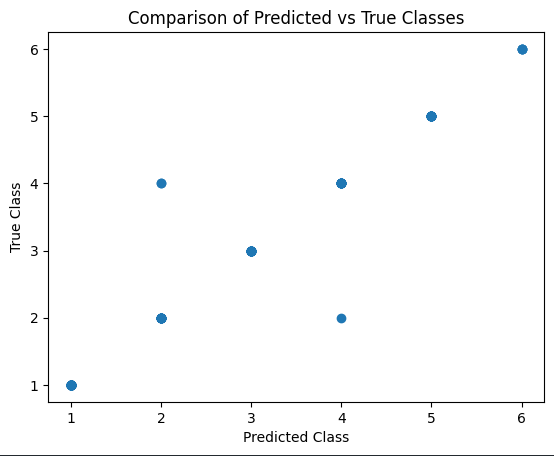
\includegraphics[width = 1.0\linewidth]{./figuras/figura4.png}}
    \caption{Gráfico de comparação de classes previstas e reais}
    \label{fig:classes}
\end{figure}

4. Gráfico de comparação de dados reais e previstos:
   - Foi plotado um gráfico de dispersão para comparar os dados reais e previstos Figura \ref{fig:dados} em relação a um dos atributos do conjunto de teste. Esse gráfico permite verificar se o modelo está capturando corretamente as relações entre os atributos e as classes, fornecendo uma visão mais detalhada do desempenho do modelo.

\begin{figure}[htbp]
    \centerline{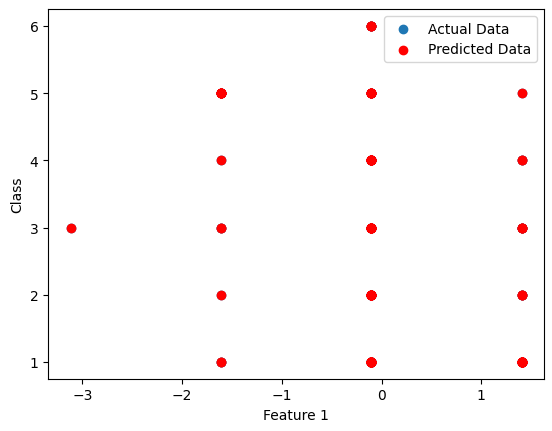
\includegraphics[width = 1.0\linewidth]{./figuras/figura5.png}}
    \caption{Gráfico de comparação de dados previstos e reais}
    \label{fig:dados}
\end{figure}

5. Matriz de confusão:
   - A matriz de confusão Figura \ref{fig:confusao} foi calculada utilizando a função 'confusion-matrix' da biblioteca scikit-learn. Essa matriz mostra a contagem de verdadeiros positivos, verdadeiros negativos, falsos positivos e falsos negativos para cada classe, permitindo uma análise mais detalhada do desempenho do modelo em termos de classificações corretas e incorretas.

\begin{figure}[htbp]
    \centerline{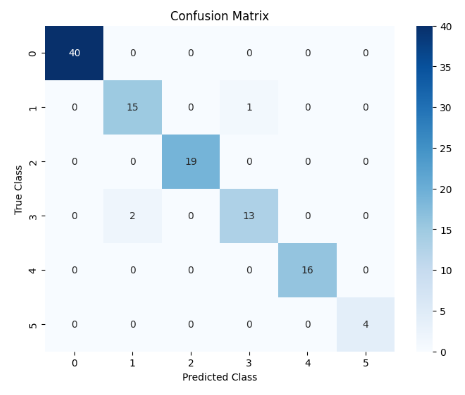
\includegraphics[width = 1.0\linewidth]{./figuras/figura6.png}}
    \caption{Matriz de confusão}
    \label{fig:confusao}
\end{figure}

6. Tabela de Métricas de Avaliação:
   - A tabela de métricas Figura \ref{fig:metricas} de avaliação foi gerada utilizando a função 'classification-report' da biblioteca scikit-learn. Essa tabela apresenta métricas como precisão, recall, F1-score e suporte para cada classe. Essas métricas fornecem uma análise mais detalhada do desempenho do modelo em cada classe, permitindo identificar classes com melhor ou pior desempenho.

\begin{figure}[htbp]
    \centerline{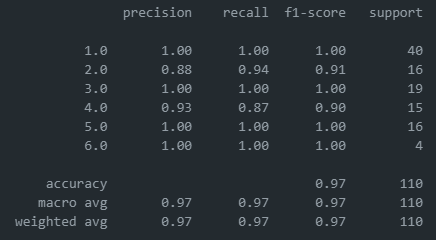
\includegraphics[width = 1.0\linewidth]{./figuras/figura7.png}}
    \caption{Tabela de métricas}
    \label{fig:metricas}
\end{figure}

Para uma futura aplicação prática do sistema é importante realizar um levantamento do histórico médico do paciente seguido por um exame físico para identificar as características importantes e fornecer os dados necessários para que a a rede neural posso gerar um resultado mais preciso, o resultado do diagnóstico resultante da análise da rede neural deve ser avaliado por um profissional capacitado para definir qual tratamento será administrado para cada paciente Figura \ref{fig:diagrama}.

\begin{figure}[htbp]
    \centerline{\includegraphics[width = 1.0\linewidth]{./figuras/figura 8.jpg}}
    \caption{Diagrama de como a rede neural pode ser utilizada para auxiliar no diagnóstico}
    \label{fig:diagrama}
\end{figure}

\section{Conclusão}
Com base nos resultados obtidos, podemos concluir que o modelo MLP implementado mostrou-se eficaz na classificação de doenças eritematoescamosas no conjunto de dados dermatológicos em comparação com o trabalho citado. A acurácia alcançada pelo modelo foi satisfatória, indicando uma taxa de classificação correta razoavelmente alta.

Os resultados positivos podem ser atribuídos a vários fatores. Primeiramente, a utilização de uma rede neural MLP permite capturar relações complexas entre os atributos e as classes, o que é crucial em problemas de classificação. Além disso, a normalização dos dados e a utilização de uma estratégia de treinamento adequada contribuíram para o bom desempenho do modelo.

Uma consideração importante sobre o experimento é a necessidade de um pré-processamento cuidadoso dos dados. A substituição dos valores ausentes e a normalização dos atributos foram etapas essenciais para garantir que o modelo funcionasse corretamente.

Para quem deseja repetir o experimento no futuro, é importante considerar algumas sugestões. Primeiramente, a exploração de diferentes arquiteturas de rede neural, incluindo variações no número de camadas e neurônios, pode ser interessante para avaliar se o desempenho do modelo pode ser melhorado. Além disso, a realização de uma busca de hiperparâmetros mais ampla pode ajudar a otimizar ainda mais o modelo.

Em relação aos trabalhos anteriores, é difícil fazer uma comparação direta, pois isso depende dos resultados específicos desses estudos. No entanto, se o modelo MLP implementado neste experimento alcançou uma acurácia superior ou comparável a esses trabalhos, pode-se considerar uma melhoria em relação a eles. 

É importante ressaltar que este experimento possui algumas limitações e dificuldades. Por exemplo, o conjunto de dados dermatológicos utilizado pode apresentar desequilíbrio de classes, o que pode afetar o desempenho do modelo. Além disso, a escolha de uma arquitetura de rede neural e hiperparâmetros específicos pode influenciar os resultados, e diferentes escolhas podem levar a desempenhos diferentes.

Sugestões de continuidade para estudos futuros incluem a expansão do conjunto de dados com mais exemplos e classes, a aplicação de técnicas de aumento de dados para lidar com o desequilíbrio de classes, a exploração de outras arquiteturas de redes neurais e a comparação com outros algoritmos de classificação. Além disso, é interessante realizar uma validação cruzada para avaliar a robustez do modelo em diferentes divisões de treinamento/teste. Também é válido investigar técnicas de interpretabilidade de modelos para compreender melhor quais características influenciam mais nas classificações.

\begin{thebibliography}{00}
\bibitem{b1} Gaurav Srivastava, Mastering ML Classifiers + Tuning [98.61 ACC]. Publicado em Kaggle.com, 2023.

\bibitem{b1} A. Boçois \textit{et al.}, "Diagnóstico de doenças dermatólogicas usando a rede neural de Kohonen", reponame: Repositório Institucional da UFPR, 2012.

\bibitem{b2} P. Gamarra Lessa Pinto, "CLASSIFICAÇÃO DE LESÕES DERMATOLÓGICAS UTILIZANDO REDES NEURAIS CONVOLUCIONAIS", in Salão de Iniciação Científica. Porto Alegre: UFRGS, 2019.

\bibitem{b3} BRAGA, Antônio de Pádua; LUDERMIR, AndréP. de  Leon F. de Carvalho e  BERNARDA, Teresa. Redes Neurais Artificiais – Teoria e Prática. 2º Edição. São Paulo: LTC, 2011. 

\bibitem{b4} CASTRO, Leandro Nunes. Computação Natural. Rio de Janeiro: Livraria da Física, 2010.

\bibitem{b5} V. A. Gulartt e R. Luiz Antoniazzi, "UTILIZAÇÃO DE REDES NEURAIS ARTIFICIAS APLICADAS NA DETECÇÃO DE MELANOMA CUTÂNEO", REVISTA INTERDISCIPLINAR DE ENSINO, PESQUISA E EXTENSÃO, vol. 8, n.º 1, p. 48–57, fevereiro de 2021.

\bibitem{b6} B. Alberto Soares Oliveira, G. Magno Moura Cardoso, F. Pereira Dias, F. Heider Willy dos Santos e F. G. Guimarães, "Sistema para Classificação de Grãos de Café: Uma Comparação entre Redes Neurais Convolucionais e Processamento Digital de Imagens com MLP", in ANAIS DO 14º SIMPÓSIO BRASILEIRO DE AUTOMAÇÃO INTELIGENTE. Ouro Preto, MG: SBAI, 2019.

\bibitem{b7} I. N. da Silva; D. H. Spatti e R. A. Flauzino, Redes Neurais Artificiais Para Engenharia e Cincias Aplicadas - Curso Pratico. ARTLIBER, 2010.

\bibitem{b8} I. Goodfellow, Y. Bengio e A. Courville, Deep Learning. MIT Press, 2016.

\bibitem{b9} I. N. da Silva, D. Hernane Spatti, R. Andrade Flauzino, L. H. B. Liboni e S. F. dos Reis Alves, Artificial Neural Networks. Cham: Springer International Publishing, 2017.

\bibitem{b10} F. Chollet, Deep Learning with Python. Manning Publications Co, 2018.

\bibitem{b11} S. Haykin, Neural Networks and Learning Machines. Pearson Education, 2009.

\bibitem{b12} DEEP LEARNING BOOK. 2022. Disponível: https://www.deeplearningbook.com.br/

\bibitem{b13} J. M. Barreto. Introdução às Redes Neurais Artificiais. Florianópolis, SC: UFSC, 2002.

\bibitem{b14} C. R. Rossini Junior; A. R. Camolesi. Um estudo no uso de Redes Neurais Artificiais associada com conceitos de Tecnologia Adaptativa na solução de problemas complexos. Assis, SP: FEMA, 2018.

\end{thebibliography}

\end{document}
